\documentclass[12pt]{article}
\usepackage[utf8]{inputenc}
\usepackage{amsmath, amssymb, amsthm}
\usepackage{graphicx}
\usepackage{caption}
\usepackage{subcaption}
\usepackage{booktabs}
\usepackage[margin=1in]{geometry}
\usepackage{enumitem}
\usepackage[colorlinks=true]{hyperref} % Improved hyperref setup

% Add this package to help with reference resolution
\usepackage{bookmark}

\title{Homework Assignment \#1}
\author{Your Name \\ Course Name}
\date{\today}

\begin{document}

\maketitle

% Add this to ensure references work properly
\phantomsection
\addcontentsline{toc}{section}{Problem 1}
\section*{Problem 1: Basic Equations}
Solve the following quadratic equation:
\begin{equation}
    ax^2 + bx + c = 0
\end{equation}

The solution is given by:
\begin{equation}
    x = \frac{-b \pm \sqrt{b^2 - 4ac}}{2a}
\end{equation}
\begin{figure}[htbp]
    \centering
    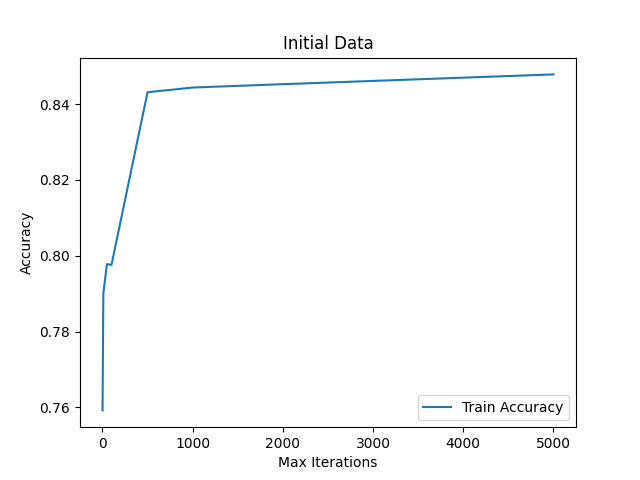
\includegraphics[width=0.5\textwidth]{test.png} % Replace with your filename
    \caption{A descriptive caption for your image}
    \label{fig:my_image}
\end{figure}
% For each section you want to reference
\phantomsection
\addcontentsline{toc}{section}{Problem 2}
\section*{Problem 2: Matrix Operations}
Given matrices \( A \) and \( B \):
\[
A = \begin{pmatrix}
1 & 2 \\
3 & 4
\end{pmatrix}, \quad
B = \begin{pmatrix}
5 & 6 \\
7 & 8
\end{pmatrix}
\]

The product \( AB \) is:
\[
AB = \begin{pmatrix}
1 \times 5 + 2 \times 7 & 1 \times 6 + 2 \times 8 \\
3 \times 5 + 4 \times 7 & 3 \times 6 + 4 \times 8
\end{pmatrix}
= \begin{pmatrix}
19 & 22 \\
43 & 50
\end{pmatrix}
\]

\phantomsection
\addcontentsline{toc}{section}{Problem 3}
\section*{Problem 3: Figure Insertion}
\begin{figure}[ht]
\centering
\includegraphics[width=0.5\textwidth]{example-image} % Make sure this image exists
\caption{Sample figure caption}
\label{fig:sample}
\end{figure}
See Figure \ref{fig:sample} for an example.

\phantomsection
\addcontentsline{toc}{section}{Problem 4}
\section*{Problem 4: Table Creation}
\begin{table}[ht]
\centering
\caption{Sample Data Table}
\label{tab:sample}
\begin{tabular}{lccr}
\toprule
Item & Quantity & Price & Total \\
\midrule
Pencils & 10 & \$0.50 & \$5.00 \\
Notebooks & 3 & \$2.00 & \$6.00 \\
Pens & 5 & \$1.50 & \$7.50 \\
\bottomrule
\end{tabular}
\end{table}
Data is shown in Table \ref{tab:sample}.

\end{document}